\makeatletter
\def\@makechapterhead#1{%
  \vspace*{10\p@}%
  {\parindent \z@ \raggedleft \normalfont
    \ifnum \c@secnumdepth >\m@ne
      \if@mainmatter
        \LARGE\bfseries \@chapapp\space \thechapter
	\vskip 4pt
        \hrule height 2pt
        \par\nobreak
        \vskip 5\p@
      \fi
    \fi
    \interlinepenalty\@M
    \huge \bfseries #1\par\nobreak
\vskip 5pt

\hrule height 2pt   
 \vskip 10\p@  
  }}
\makeatother

\setcounter{chapter}{8}
\chapter{Transducers}\label{chap9}
\addtocontents{toc}{\protect\contentsline{chapter}{\protect Chapter \numberline{\thechapter.}
Transducers}{\thepage--\pageref{9end}}}  

\section{Introduction}\label{sec9.1}%% 9.1
A transducer is a device which converts energy from one form to
another form. The energy may be electrical, mechanical chemical,
thermal or optical.

A generalized measurement system consists of three major parts 
\begin{itemize}
\item[(i)] an input device
\item[(ii)] a signal conditioning or processing device \&
\item[(iii)] an output device.
\end{itemize}

The input device receives the measurand (physical quantity to be
measured) and delivers a proportional or analogous electrical signal
to the signal conditioning or processing device where the signal is
amplified, attenuated, filtered  modulated  or modified in to a form
acceptable by the output device examples for some of the physical
quantites are heat, light intensity, pressure, humidity, liquid level,
PH value etc. These physical quantities may be converted into
electrical form (voltage, et. frequency) by means of transducers
called electrical transducers. The electrical output generated by the
electrical transducer is measured by standard method which gives the
magnitude of the \& input physical quantity in terms of analogous
electrical output.

\section{Electrical Transducer}\label{sec9.2}
An electrical transducer is a sensing device by which the physical
quantity to be measured  is transformed into an electrical output
(voltage, current or frequency) proportional to the input measurand
by a suitable mechanism.  Basically an electric transducer consists of
two important and closely related elements as shown in
Fig.~\ref{fig9.1} below.

These two parts are (i) Sensing element or detector \& (ii)
Transduction element.

In order to measure a non-electrical physical quantity a sensing
element or detector is used which usually converts the physical
quantity to be measured  into a displacement. This displacement
actuates  a transduction element which gives an output which is
electric in nature. Thus the transduction elements acts a secondary
transducer. The electric output may be voltage, current or frequency
and the production of these outputs is based upon  the electrocal
effects which may be resistive, capacitive, inductive etc in nature.
\begin{figure}[H]
\centering
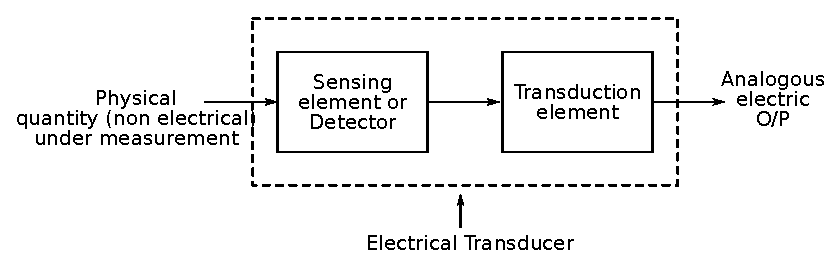
\includegraphics{chap9/fig9.1.eps}
\caption{Elements of basic electrical transducer.}\label{fig9.1}
\end{figure}

\section{Characteristics of Electric Transducers:}\label{sec9.3}

The selected transducers for any measurement system possess the
following characteristics :
\begin{itemize}
\item[(i)] Mechanical ruggedness : The transducer must be mechanically
  rugged i.e., it must be able to withstand the working conditions and
  mechanical strains.

\item[(ii)] Linear input/output characteristic : The transducers must
  have linear input/output characteristics.

\item[(iii)] Sensitivity to measurand : Must be very sensitive to the
  change in the measurand i.e., physical quantity to be measured. 

\item[(iv)] Low noise : Must exhibit minimum sensitivity to noise i.e.,
  signal to noise ratio of the transducer must be low.

\item[(v)] Accuracy : Must be accurate against the error due to
  calibration and other stimuli.

\item[(vi)] Reliability : The output of the transducer must be
  reliable. The result must be stable and should not change with
  temperature and other changes.

\item[(vii)] Frequency response : The frequency response of the
  transducer must be flat over the entire desired frequency range.

\item[(viii)] Physical size : The transducer must have minimal weight
  and size, so that its presence in the measurement system doesnot
  disturb the existing conditions.
\end{itemize}

\section{Classification of electrical transducers}\label{sec9.4}

The electrical transducers can be classified as 
\begin{enumerate}
\item[(a)] Active and Passive transducers :
\begin{itemize}
\item[(i)] Active transducers: These transducers develop electrical
  output (voltage, current or frequency) of their own. For this, they
  obtain energy from the physical quantity being measured.

Eg. : Thermocouples, piezoelectric transducer, photo voltaic cell,
photoelectric cell etc.
 
\item[(ii)] Passive transducers: These transducers do not develop
  electrical output of their own and need as external power or energy
  source for the purpose.

Eg. : Strain gauges, themistor, LVDT, Hall effect generator etc.
\end{itemize}

\item[(b)] Primary and Secondary transducers :
\begin{itemize}
\item[(i)] Primary transducers: These converest the physical quantity
  to be measured directly into electrical output after sensing or
  detecting the quantity 

Eg. : thermocouples.  

\item[(ii)] Secondary transducers : Conversion from physical quantity
  into electrical output is done first by sensing the quantity and
  then converting it into electrical output.

Eg. : LVDT etc.
\end{itemize}

\item[(c)] Analog and Digital transducers :
\begin{itemize}
\item[(i)] Analog transducers : These transducers convert the input
  physical quantity into an electric output which is a continuous
  function of time (a i.e., analog)

Eg. : Strain gouge, LVDT, thermocouple, thermistor etc.

\item[(ii)] Digital transducers : There transducers converts the input
  physical quantity into an electric output which is in the form of
  pulses (i.e., digital)

Eg. : Class seals, metal seals etc.
\end{itemize}
\end{enumerate}

\eject

\section{Advantages of electric Transducer}\label{sec9.5}

The advantages of converting physical quantities into an analogous
electrical quantities are
\begin{itemize}
\item[(i)] Electrical amplification and attennation can be alone easily.

\item[(ii)] Mass-inertia effects are minimised 

\item[(iii)] The effects of friction are minimised

\item[(iv)] The electrical measurement systems can be controlled with
  a very small power.

\item[(v)] The output can be indicated and recorded remotely at a
  distance from the sensing element.

\item[(vi)] The electrical output signal can be easily used,
  transmitted and processed for the measurement.

\item[(vii)] Since electronic components and devices amenable to
  miniaturization, electrical transducers are better option for a
  measurement system. 
\end{itemize}


\section{Passive Electrical Transducers}\label{sec9.6}

These transducers donot  develop electrical output of their own and
need an external power or energy source for the purpose. Depending on
the electrical phenomena employed in the transduction elements of
transducers, we have the following types of passive electrical
transducers.
\begin{itemize}
\item[(i)] Resistive transducers  ~Eg : Resistance thermometer,
Thermistor Strain gauge etc.

\item[(ii)] Inductive transducers ~Eg : LVDT, Magnetostriction gauge
etc. 

\item[(iii)] Capacitive transducers ~Eg : Capacitance pressure gange,
microphone etc.

\item[(iv)] Voltage or current transducers ~Eg : \& Hall effect
generator, photomissive all, photomultiplier tube etc.
\end{itemize}

Among the examples given above only resistive transducers (Resistance
thermometer \& thermistor) and inductive transducer (Linear variable
differential transformer i.e., LVDT) are discussed in the following sections.

\subsection{Resistive Transducers}\label{sec9.6.1}

The resistance of a metal conductor is given by, 
\begin{equation}
\rmR = \dfrac{\rho\rml}{\rmA} \label{eq9.1}
\end{equation}
\begin{tabbing}
where ~~R \= = \= resistance of the conductor  ($\Omega$)\\[3pt]
\quad\qquad~ l \> = \> length of the conductor (m)\\[3pt]
\quad\qquad~A \> = \> cross-sectional area the conductor (m$^2$)\\[3pt]
\quad\qquad~$\rho$ \> = \> resistivity of the conductor ($\Omega~ -\rmm$)
\end{tabbing}

Any method of varying one of the quantities in Eqn.~\eqref{eq9.1}
[i.e., $\rho$, l, and A] is the design basis of an electrical resistive
transducer. There are a number of methods by which resistance can be
changed by a physical phenomenon. For example,
\begin{itemize}
\item[(a)] a potentiometer can be used for measurement of
displacements as it resistance changes with change in length of its
conductor 
\item[(b)] a straingauge can be used for measurement of force and
pressure as its resistance changes when it is strained and 
\item[(c)] a material can be used for measurement of temperature as
its resistivity changes with temperature.
\end{itemize}

\subsubsection{Principle Resistance thermometers}\label{sec9.6.1.1}
When the temperature is changed, the resistance of a conductor changes
because its resistivity $\rho$ and length l changes. This property is
utilized for measurement of temperature. A conductor has positive
temperature coefficient of resistance (i.e., as temperature increases
the resistance also increases) and is given by, 
\begin{equation}
\alpha = \frac{1}{\Delta \rmT} \cdot \frac{\Delta \rmR}{\rmR_o}\label{eq9.2}
\end{equation}
\begin{tabbing}
where ~~~$\Delta$T \= = \= change in temperature ($^\circ$C) \\[3pt]
\qquad \quad~$\dfrac{\Delta \rmR}{\rmR_0}$ \> = \> fractional change in resistance \\[3pt]
\qquad \quad~ $\rmR_0$ \> = \> resistance at $0^\circ$ C ($\Omega$)
\end{tabbing}

The resistance $\rmR_\rmT$ at any other temperature T$^\circ$C is
given by 
\begin{equation}
\rmT = \rmR_0 (1+\alpha \rmT) \label{eq9.3}
\end{equation}

Also by linear approximation (R Vs T is linear), the resistance
$\rmR_\rmT$ at a temperature T$^\circ$C is given by
$$
\rmR_\rmT = \rmR_{\rmT_0}
(1+ \alpha_{\rmT_0} \Delta \rmT) \quad \text{ with } \quad \theta_1
< \theta_0 < \theta_2
$$
\begin{tabbing}
where ~~$\rmR_{\rmT_0}$ \= = \= approximate resistance at T$^\circ_0$C
($\Omega$)\\[4pt]
\qquad\quad ~$\Delta$T \> = \> $\rmT-\rmT_0$ = change in temperature ($^\circ$C),\\[4pt]
\qquad \quad ~$\alpha_{\rmT_0}$ \> = \> temperature coefficient of resistance at
temperature T$_0^\circ$C (/$^\circ$C).
\end{tabbing}

\heading{Characteristics of conducting material:}

 The requirements of a conducting material to be used in resistance
 thermometers are,
\begin{itemize}
\item[(i)] The change in resistance of conducting material per unit
 change in temperature must be as large as possible.

\item[(ii)] The conducting material must have a high value of
resistivity so that minimum volume of conductor material is used

\item[(iii)] The resistance of conducting materials must have a stable
relationship with temperature.
\end{itemize}

The most commonly used conducting material in resistance thermometer
is platinum\break because it 
\begin{itemize}
\item[(a)] can withstand high temperatures. 

\item[(b)] maintains excellent stability.

\item[(c)] shows minimum susceptibility to contamination.
\end{itemize}

The other conducting materials used in resistance thermometer are
copper, Nickel, Tungsten etc.

\heading{Construction}

The wire resistance thermometers are as shown in Fig.~\ref{fig9.2}(a) \&\ (b) below.

It consist of a platinum coil wound on a mica or ceramic strip which
also acts as a supporting  mount for the coil. This is enclosed in a
protective tube made of pyrex glass, porcelain, guartz etc. The two
terminals of the coil are brought to contact with the substances
(usually fluid) whose temperature is to be measured. Then the
terminal of the coil is connected to as arm of wheatstone bridge for
measuring the change in resistance so that the temperature can be
measured using Eqn.~\eqref{eq9.3}.
\begin{figure}[H]
\centering
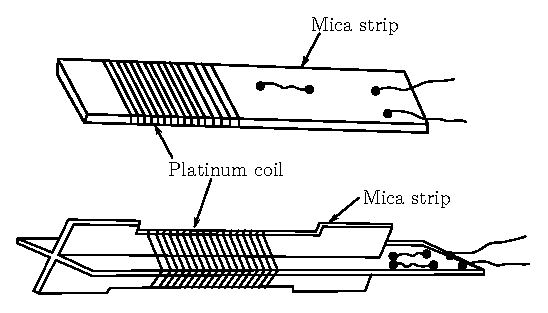
\includegraphics{chap9/fig9.1a.eps}
\caption{Resistance thermometer}\label{fig9.2}
\end{figure}

\begin{center}
\rule{4cm}{1pt}\\
{\bf\Large Problems}\\[-3pt]
\rule{4cm}{1pt}
\end{center}

\begin{problem}\label{prob9.1}
A platinum thermometer has a resistance of 100 $\Omega$ at $25^\circ$C.
\begin{itemize}
\item[(a)] Find its resistance at 65$^\circ$C if the platinum has a
temperature coefficient of resistance 0.00392/$^\circ$C.

\item[(b)] If the thermometer has a resistance of 150 $\Omega$,
calculate the temperature.
\end{itemize}
\end{problem}

\begin{solution}
We have
$$
\rmR_\rmT = \rmR_{\rmT_0} \left(1 + \alpha_{\rmT_0} \Delta \rmT\right)
$$
\begin{tabbing}
Given ~~$\rmR_{\rmT_0}$ \= = \= resistance at 25$^\circ$C = 100 $\Omega$\\[4pt]
\qquad \quad~$\Delta$T \>  = \> T - T$_0$ = change in temperature = 65 -25 = 40$^\circ$C\\[4pt]
\qquad \quad~$\alpha_{\rmT_0}$ \> = \> temperature coefficient of resistance at
65$^\circ$C  = 0.00392/$^\circ$C.
\end{tabbing}
\begin{tabbing}
$\therefore$ Resistance at ~65$^\circ$C \= = \= $\rmR_\rmT = \rmR_{\rmT_0}
(1+ \alpha_{\rmT_0} \Delta \rmT)$\\[3pt]
\> = \> $100 (1+0.00392 \times 40)$\\[3pt]
\> = \> 115.68 $\Omega$.
\end{tabbing}

Let T be the unknown resistance.
\begin{align*}
\therefore \quad 150 & = 100 \left[1+ 0.00392 (\rmT -25) \right]\\[3pt]
\therefore \quad \rmT & = 152.55^\circ \rmC
\end{align*}
\end{solution}

\subsubsection{Thermistors}\label{sec9.6.1.2}
Thermistors (\textit{thermal resistors}) are generally composed of
semi-conductor materials and it exhibits negative temperature
coefficient of resistance (i.e. resistance decreases as temperature
increases) with value of 3.5\% per $^\circ$C makes it to detect very
small changes in temperature which is not possible using resistance
thermometer. The high sensitivity to temperature changes makes
thermistors extremely useful for precission measurements.

The resistance of thermistors ranges from 0.5 $\Omega$ to 0.75
M$\Omega$ and they are widely used in applications which involve
measurements in the range of $-60^\circ$C to $15^\circ$C. Even though
thermistors are highly sensitive to temperature variation, the
drawback is they exhibit highly non-linear characteristic of
resistance versus temperature. 

\heading{Construction:} Thermistors are made up of sintered mixture of
metallic oxides such as cobalt, nickel, manganese, copper, iron and
uranium. They are available in different sizes and shapes. They may be
in the form of beads, probes, rods and discs as shown in
Fig.~\ref{fig9.3} below.
\begin{figure}[H]
\centering
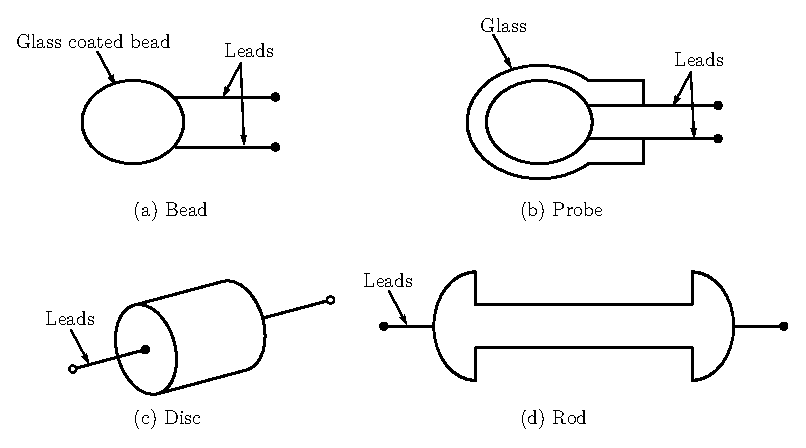
\includegraphics[scale=.97]{chap9/fig9.2.eps}
\caption{Different forms of construction of thermistors}\label{fig9.3}
\end{figure}

The circuit symbol of thermistor is shown in Fig.~\ref{eq9.4} below.
\begin{figure}[H]
\centering

\includegraphics[scale=.97]{chap9/fig9.3.eps}
\caption{Symbol of thermistorn}\label{fig9.4}
\end{figure}

\vfill\eject

\heading{Resistance-Temperature characteristics:}

The relationship between the resistance of a thermistor and
temperature of thermistor is give by,
\begin{equation}
R_{T_1} = R_{T_2} \text{ exp } \left[\beta \left(\dfrac{1}{T_1}
- \dfrac{1}{T_2} \right) \right] \label{eq9.4}
\end{equation}
\begin{tabbing}
\text{where } ~~R$_{\rmT_1}$ \= = \=  resistance of the thermistor at
temperature T$_1^\circ$k. ($\Omega$)\\[4pt]
\qquad\quad~ R$_{\rmT_2}$ \> = \> resistance of the thermistor at  temperature
T$^\circ_2$k. ($\Omega$)\\[4pt]
\quad\quad \& ~~ $\beta$ \> = \> ma constant depending upon the material of
thermistor\\[4pt]
\> \> \quad  (typical value 3500 to 4500$^\circ$k).
\end{tabbing}

\begin{problem}\label{prob9.2}
A thermistor has a resistance of 3.98 k$\Omega$ at the ice point
(0$^\circ$C) and 794 $\Omega$ at 50$^\circ$C ~(i) Find the constant
$\beta$ of thermistor (ii) calculate the range of resistance
variation, if the temperature varies from 40$^\circ$C to 100$^\circ$C.
\end{problem}

\begin{solution}
\begin{itemize}
\item[(i)] Given ~~$\rmR_{\rmT_1} =3.98$ k$\Omega$ ~~$\rmR_{\rmT_2} =794\Omega$
\begin{tabbing}
$\rmT_1 =0^\circ$C \quad $\therefore$~ ~$\rmT_1$ \= = \= $(0+273)^\circ$ k =
$273^\circ$ k.\\[7pt]
$\rmT_2 = 50^\circ$C \quad~~ $\rmT_2$ \> = \> $(50+273)$ k = $323^\circ$
k.\\[7pt]
We have \quad \quad~~$\rmR_{\rmT_1}$ \> = \>
$\rmR_{\rmT_2} \exp \left[\beta\left(\dfrac{1}{\rmT_1}
- \dfrac{1}{\rmT_2} \right)\right]$ \\[0.25cm]
\hspace{2cm} 3980 \> = \> 794 $\exp \left[\beta\left(\dfrac{1}{273}
-\dfrac{1}{323} \right) \right]$\\[7pt]
\hspace{2cm} $\therefore $ ~ $\beta$ \> = \> 2843
\end{tabbing}
when $\rmT_2 =40^\circ$C;

\item[(ii)] Take $\rmT_1 =0^\circ$C = 273$^\circ$ k \quad $\therefore$ ~
Given $\rmT_2 = 40^\circ$C = $40 + 273=313^\circ$ k
\begin{gather*}
\therefore \quad 3980
= \rmR_{\rmT_2} \exp \left[2843 \left(\frac{1}{273}
- \frac{1}{313} \right) \right]\quad \\[4pt]
\therefore \rmR_{\rmT_2} = 1051~ \Omega
\end{gather*}
when $\rmT_2 = 100^\circ$C

\eject

Take $\rmT_1=0^\circ$C = 273$^\circ$k \quad $\therefore$~ Given
$\rmT_2 = 100^\circ$C = 100 + 273 = 373$^\circ$ k

\smallskip
$\therefore$ ~ 3980 = $\rmR_{\rmT_2} \exp \left[2843 \left(\dfrac{1}{273}
- \dfrac{1}{373} \right) \right]$

\smallskip
$\therefore$ ~ $\rmR_{\rmT_2} \simeq 244\Omega$ ~~[$\therefore$ The range of
resistance is 244$\Omega$ to 1051$\Omega$]
\end{itemize}
\end{solution}

\subsection{Inductive Transsucers}\label{sec9.6.2}
Generally, inductive transducers work upon the following principles.
\begin{itemize}
\item[(i)] Change of self inductance

\item[(ii)] Change of mutual inductance
\end{itemize}
\begin{itemize}
\item[(i)] \textbf{Change of self inductance :} The self inductance of
a coil is given by,
\begin{equation}
\rmL = \frac{\rmN^2 \mu \rmA}{\rml} \label{eq9.5}
\end{equation}
\begin{tabbing}
where ~~ N \= = \= number of turns.\\[3pt]
\qquad \quad~ $\mu$ \> = \> permeability of medium in and around the coil : ($\mu$/m)\\[3pt]
\qquad \quad~ A \> = \> area of cross section of coil ($\rmm^2$)\\[3pt]
\qquad \quad~ l \> = \> length of coil (m).
\end{tabbing}

Eqn.~\eqref{eq9.5} indicates that the variation of self inductance
takes place if,
\begin{itemize}
\item[(i)] the number of turns N changes.

\item[(ii)] the geometric size i.e., A or l changes.

\item[(iii)] the permeability $\mu$ changes.
\end{itemize}

The physical quantity (usually displacement) to be measured is
arranged to cause variation of any of the above three variables in
Eqn.~\eqref{eq9.5} which alters the self inductance. This variation in
self inductance may be used for measurement of a physical quantity.

\item[(ii)] \textbf{Change of mutual inductance :} The mutual
inductance between two coils is given by,
\begin{equation}
\rmM = \rmk \sqrt{\rmL_1 \rmL_2} \label{eq9.6}
\end{equation}
\begin{tabbing}
where ~ $\rmL_1$ \= = \= self inductance of first coil.\\[3pt]
\qquad ~~ ~ $\rmL_2$ \> = \> self inductance of second coil.\\[3pt]
\qquad ~~ ~ k \>  = \> Coupling coefficient 
\end{tabbing}
\end{itemize}

\vfill\eject

Eqn.~\eqref{eq9.6} indicates that the mutual inductance between two
coils can be varied by changing the self inductances
($\rmL_1 ~\&~ \rmL_2$) or the coupling coefficient (\rmM). This
variation of mutual inductance may be used for measurement of a
physical quantity (usually displacement).

An inductive transducers called Linear Variable Differential
Transformer (LVDT) which works on the principle of change of mutual
inductance is discussed in the next section.

\subsection{Linear Variable Differential Transformed (LVDT)}\label{sec9.6.3}

The most widely used inductive transducer to transform a linear motion
(displacement) into electrical signal is linear variable differential
transformer (LVDT). The constructional diagram of LVDT us shown in
Fig.~\ref{fig9.4} below.
\begin{figure}[H]
\centering
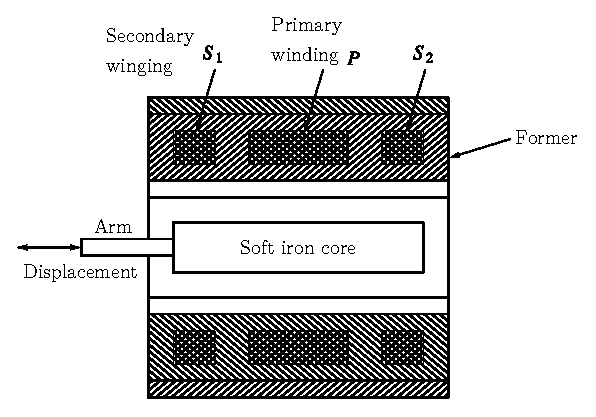
\includegraphics[scale=1.15]{chap9/fig9.3a.eps}

\medskip
\caption{Construction of Linear Variable Differential Transformer (LVDT)}\label{fig9.5}
\end{figure}

This transformer consists of single primary winding $P$ and two
secondary windings S$_1$ and S$_2$ which have equal number of turns
and are identically placed on either side of the primary winding. The
primary winding is excited by an alternating current source. Both the
windings (P and $\rmS_1 ~\&~ \rmS_2$) are wound on a cylindrical former. A
movable soft iron core is placed inside the former which is free to
move inside the coil in either direction from the central (null)
position. Usually the core is made of high permeability nickel
iron. The entire assembly is placed in a stainless steel housing which
provides electrostatic and electromagnetic shielding.

The excitation of primary winding with an alternating current source
produces an alternating magnetic field which in turn induces
alternating voltage in the two secondary windings. 

The circuit symbol of LVDT is shown in Fig.~\ref{fig9.6} below.
\begin{figure}[H]
\centering
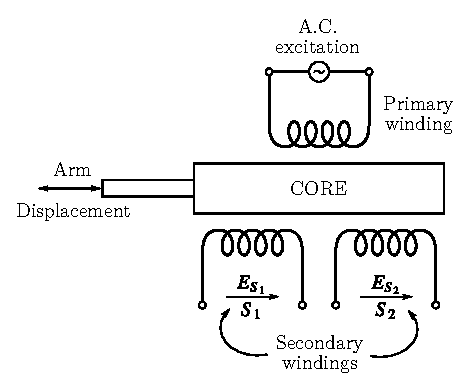
\includegraphics{chap9/fig9.4.eps}
\caption{Circuits of LVDT}\label{fig9.6}
\end{figure}

\heading{Operation :} The operation of LVDT may be explained with the
help of Fig.~\ref{fig9.7} shown below.
\begin{figure}[H]
\centering
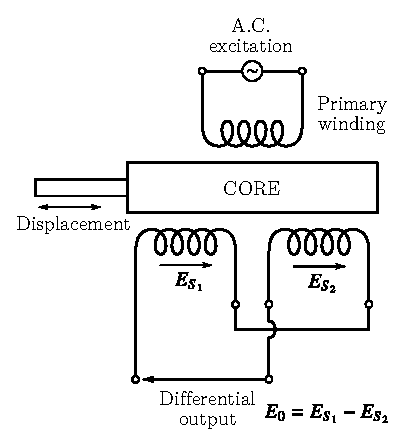
\includegraphics{chap9/fig9.5.eps}
\caption{Working of LVDT}\label{fig9.7}
\end{figure}

Let~~ $\rmE_{\rmS_1}$ = output voltage of secondary $\rmS_1$

\smallskip
\qquad $\rmE_{\rmS_2}$ = output voltage of secondary $\rmS_1$.

\smallskip
In order to convert the outputs of from $\rmS_1$ and $\rmS_2$ into a single
voltage, $\rmS_1$ and $\rmS_2$ are connected in oppositely series on shown
in Fig.~\ref{fig9.6}. Thus the output voltage $\rmE_0$ of the transducer
is the difference of the two voltages $\rmE_{\rmS_1}$ and $\rmE_{\rmS_2}$.

\smallskip
i.e., the differential output voltage,
\begin{equation}
\rmE_0 = \rmE_{\rmS_1} - \rmE_{\rmS_2} \label{eq9.7}
\end{equation}

When the core is at its normal or null position, the magnetic flux
linting with both $\rmS_1$ and $\rmS_2$ is equal. $\therefore$~~
$\rmE_{\rmS_1} = \rmE_{\rmS_2}$ \quad $\therefore ~ \rmE_0 = 0$ at
null position.

\smallskip
If the core is moved to the left of the null position, the magnetic
flux linking with $\rmS_1$ is more than that with
$\rmS_2$. i.e., ~$\rmE_{\rmS_1} > \rmE_{\rmS_2}$.~ ~~$\therefore$~ $\rmE_0=
\rmE_{\rmS_1} - \rmE_{\rmS_2} > 0$ (positive) 

\smallskip
Thus the output voltage $\rmE_0$ is in phase with the primary voltage.

\smallskip
Similarly, if the core is moved to the right of the null position, the
magnetic flux linking with S$_2$ is more than that with ~S$_1$ i.e.,
~~$\rmE_{\rmS_2} > \rmE_{\rmS_1}$,~~ ~$\therefore$~ $\rmE_0 = \rmE_{\rmS_1} -
\rmE_{\rmS_2} < 0$ (negative) 

\smallskip
Thus the output voltage $\rmE_0$ is out of phase with the primary
voltage.

\smallskip
This amount of output voltage is measured to determine a physical
quantity (displacement). The graph of output voltage $\rmE_0$ of an
LVDT verses core displacement is shown in Fig.~\ref{fig9.8} below.
\begin{figure}[H]
\centering
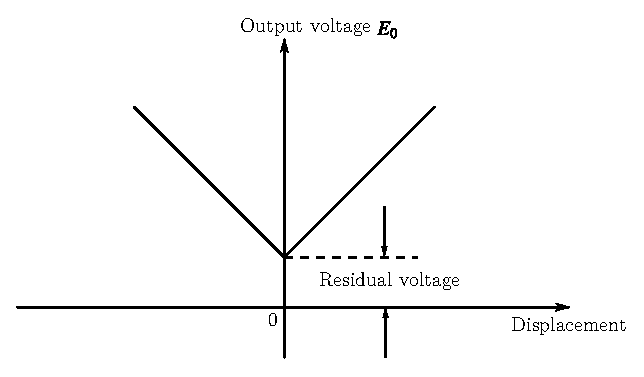
\includegraphics{chap9/fig9.6.eps}
\caption{Output Voltage \boldmath{$\rmE_0$} Vs core displacement.}\label{fig9.8}
\end{figure}

\eject

Ideally the output voltage $\rmE_0$ at the null position must be equal to
zero. But practically, there exists a small output voltage at the
null position due to.
\begin{itemize}
\item[(i)] the presence of harmonics in the input supply voltage

\item[(ii)] the harmonics produced in the output voltage which
results due to the usage of iron core.

\item[(iii)] the incompletion of either  magnetic or electrical
unbalance or both.
\end{itemize}

\heading{Advantages of LVDT :}
\begin{itemize}
\item[(i)] The LVDT have a very high range for measurement of
displacement (typically ranging from 1mm to 250 mm).

\item[(ii)] Frictionless : As there is no physical contact between the
movable iron core and transformer windings, LVDT is frictionless.

\item[(iii)] Electrical isolation : The seperation between iron core
and transformer windings permits the electrical isolation between the
iron core and transformer windings. 

\item[(iv)] High sensitivity : LVDT gives a high output even for a
small displacement which may not require amplification.

\item[(v)] Ruggedness : LVDT can tolerate high degree of shock and
vibrations without any adverse effects.

\item[(vi)] Low Hysterisis : The repeatability of LVDT is excellent as
it exhibits low hysterisis.

\item[(vii)] Low power consumption : Consumer less power which is
usually less than 1 W.
\end{itemize}


\heading{Disadvantages of LVDT :}
\begin{itemize}
\item[(i)] LVDTs are sensitive to Stray magnetic fields.

\item[(ii)] The receiving instrument connected to the output of LVDT
must operate on ac voltage or current.

\item[(iii)] The performance of LVDT depends mechanically on the man
of the iron core and electrically on the frequency of the applied voltage.

\item[(iv)] Temperature affects the performance of an LVDT.
\end{itemize}

\section{Active Electrical Transducers}\label{sec9.7}

These transducers develop electrical output (voltage, current or
frequency) of their own. For this, they obtain energy from the
physical quantity being measured. Examples are piezoelectric
transducers, thermocouples, thermopiles photoelectric transducer etc.

Among the examples given above only piezoelectric and photoelectric
transducers are discussed in the following sections.

\subsection{Piezoelectric transducers}\label{sec9.7.1}

A piezoelectric material is a crystal that producers an electric
potential (emf) across its surfaces when it is subjected to a
mechanical force. The emf generated is due to the displacement of
charges. This effect is reversible. i.e., if a varying  emf is applied
across piezoelectric  material it will change the dimension of the
crystal.

This effect is known piezoelectric effect.

Piezoelectric materials may be natural or synthetic. Examples for
piezoelectric materials are Rochelle salt, ammonium dihydrogen
phosphate lithium sulphate, quantz ceramics etc. Among these Rochelle
salt and quartz are popular because they are available naturally.

Piezoelectric transducers have high mechanical rigidity so that it may
be used to measure force, pressure, torque, strain, vibrations etc.

The magnitude and polarity of the induced emf are proportional to the
magnitude and direction of the applied mechanical force.

A piezoelectric crystal subjected to mechanical force shown in
Fig.~\ref{fig9.9} below.
\begin{figure}[H]
\begin{minipage}[b]{7cm}
\centering
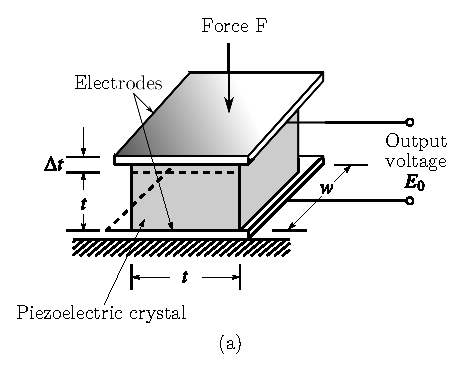
\includegraphics{chap9/fig9.7a.eps}
\end{minipage}
\qquad
\begin{minipage}[b]{6.5cm}
\centering
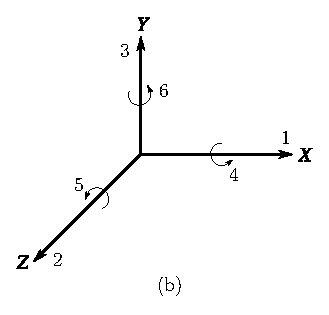
\includegraphics{chap9/fig9.7b.eps}
\end{minipage}
\caption{A piezoelectric crystal subjected to machanical force.}\label{fig9.9}
\end{figure}

The piezoelectric effect is direction sensitive. For example, if a
tensile force produces a voltage of one polarity, the compressive
force produces a voltage of opposite polarity.

The piezoelectric crystals are used in many modes. These modes are (i)
Thickness expander (ii)  Transverse  expander (iii) Thickness shear
(iv) Face shear. They are shown in Fig.~\ref{fig9.10} (a), (b), (c) and
(d) respectively.
\begin{figure}[H]
\centering
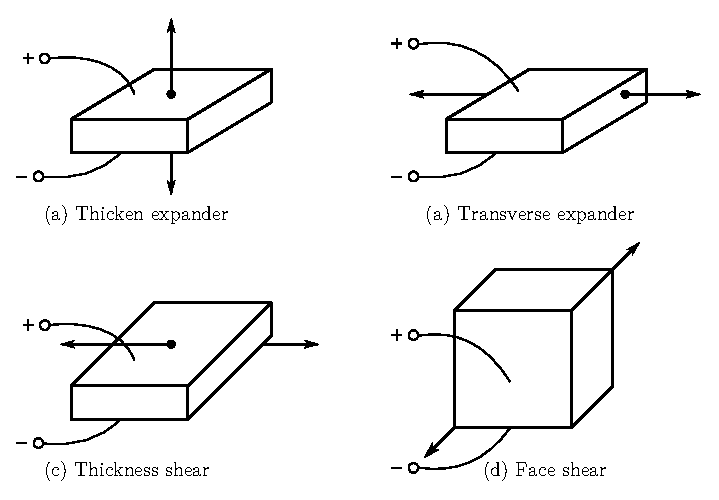
\includegraphics{chap9/fig9.8.eps}
\caption{Different modes of operation of piezoelectric crystals}\label{fig9.10}
\end{figure}

\heading{Equivalent Circuit of Piezoelectric Crystal}

The basic equivalent circuit of a piezoelectric transducer is shown in
Fig.~\ref{fig9.11} (a) \& (b) below.
\begin{figure}[H]
\centering
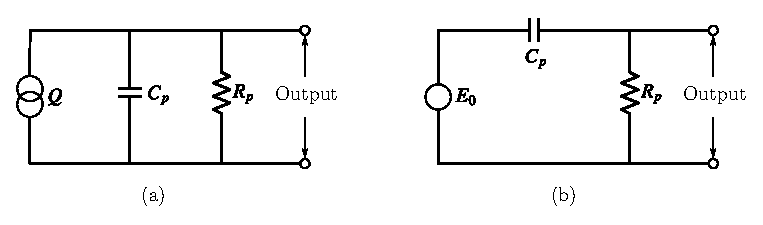
\includegraphics{chap9/fig9.9.eps}
\caption{Equivalent circuit of piezoelectric crystal.}\label{fig9.11}
\end{figure}

The source of output emf $\rmE_0$ is the generation of charge across
the surface of the crystal. Its value is given by
\begin{equation}
\rmQ=\rmd\rmF \label{eq9.8}
\end{equation}
\begin{tabbing}
where ~d \= = \= charge sensitivity of the crystal (C/N)\\[4pt]
\> \>  It is constant for a given crystal.\\[4pt]
\qquad \quad F \> = \> applied mechanical force (N).
\end{tabbing}

The charge is generated across the capacitance C$_\rmP$ of the crystal
and its leakage resistance R$_\rmP$.

The charge generator can be replaced by an equivalent voltage source
E$_0$ as shown in Fig.~\ref{fig9.9}(b) and is given by 
\begin{equation}
\rmE_0 = \dfrac{\rmQ}{\rmC_\rmP}  = \dfrac{\rmd\rmF}{\rmC_\rmP} \label{eq9.9}
\end{equation}

\subsection{Photoelectric Transducers}\label{sec9.7.2}
`Opto-electronics' is the branch of electronics, which deals with the
light sensitive devices. When light energy is incident on
optoelectronic devices, it generates an electric current in the
devices. The opto-electronic devices work on the basis of
`photo-electric effect'. Therefore these devices are called
photoelectric devices or photoelectric transducers. 

A photoelectric transducer is based on the effects of light radiation
on electrons. If light energy falls on an electron bound in a metal
surface or semiconductor, the entire quantum energy (light energy) is
converted into kinetic energy of the electron. This kinetic energy
results in the movement of electrons and thereby current in the metal
or semiconductor. This is called `photoelectric effect' i.e., the
effect of light radiation on the metal or semiconductor.

The different forms of photoelectric effect are, 
\begin{itemize}
\item[(i)] Photoemissive  effect : It causes due to the liberation of
electrons from a metallic surface under the influence of light. Eg. :
Vaccuum and gas tubes, photo FET etc.

\item[(ii)] Photoconductive effect : This effect is the result of the
dependancy of electrical conductivity of a semiconductor bar on the
intensity of light falling on it. Eg. : Photo resistor. 

\item[(iii)] Photovoltaic  effect : This effect is the result of the
generation of emf across a reverse biased PN junction under the
influence of light. Eg. : Photo diode, photo transistor, photo SCR etc.
\end{itemize}

\label{9end}
